\section{Payload Systems and Operation}
\label{sec:Hardware}

\begin{figure}[!ht]
\begin{center}
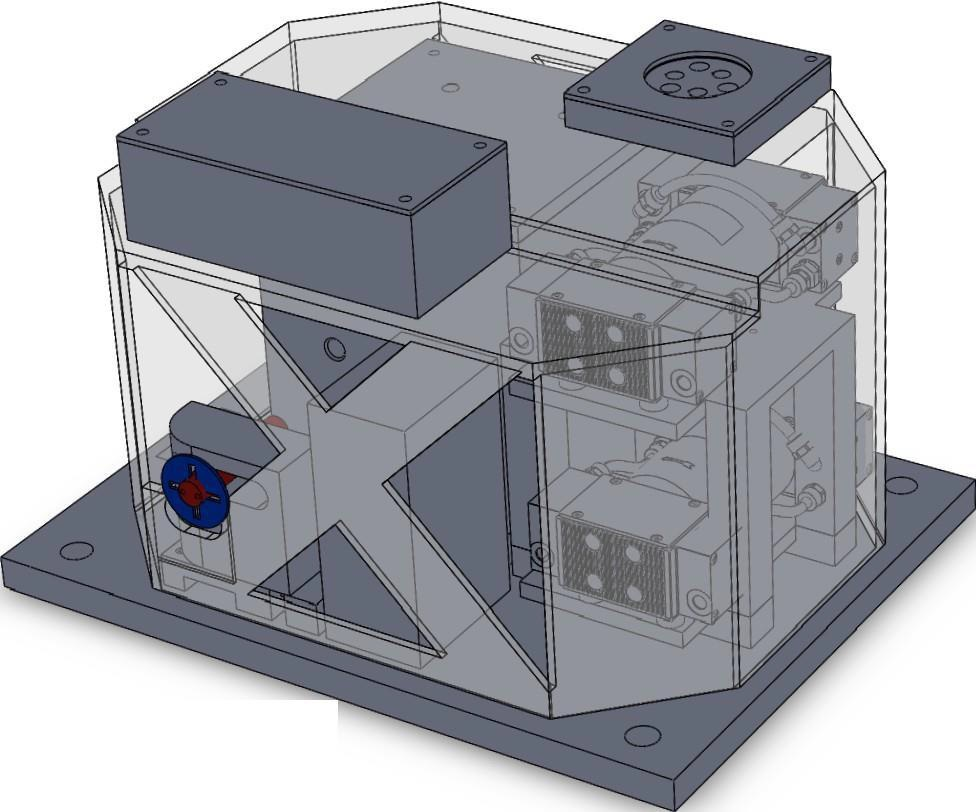
\includegraphics[width=.75\textwidth]{./Figures/payload_1.jpg}
\caption{SolidWorks 3D CAD design of the SORA payload.}
\label{fig:payload} 
\end{center}
\end{figure}

The SORA 2.0 payload will have an upgraded and more efficient flight computer, a fully developed astrobiology system and a MiniPIX USB silicon-based hybrid-chip particle detector.  The astrobiology system will build upon the previous mission, but this time we are seeking to capture and culture any microorganisms we may find.  Our previous mission in 2017 confirmed that our astrobiology system functions well beyond expectations and that there are microorganisms in the upper atmosphere.

\begin{figure}[!ht]
\begin{center}
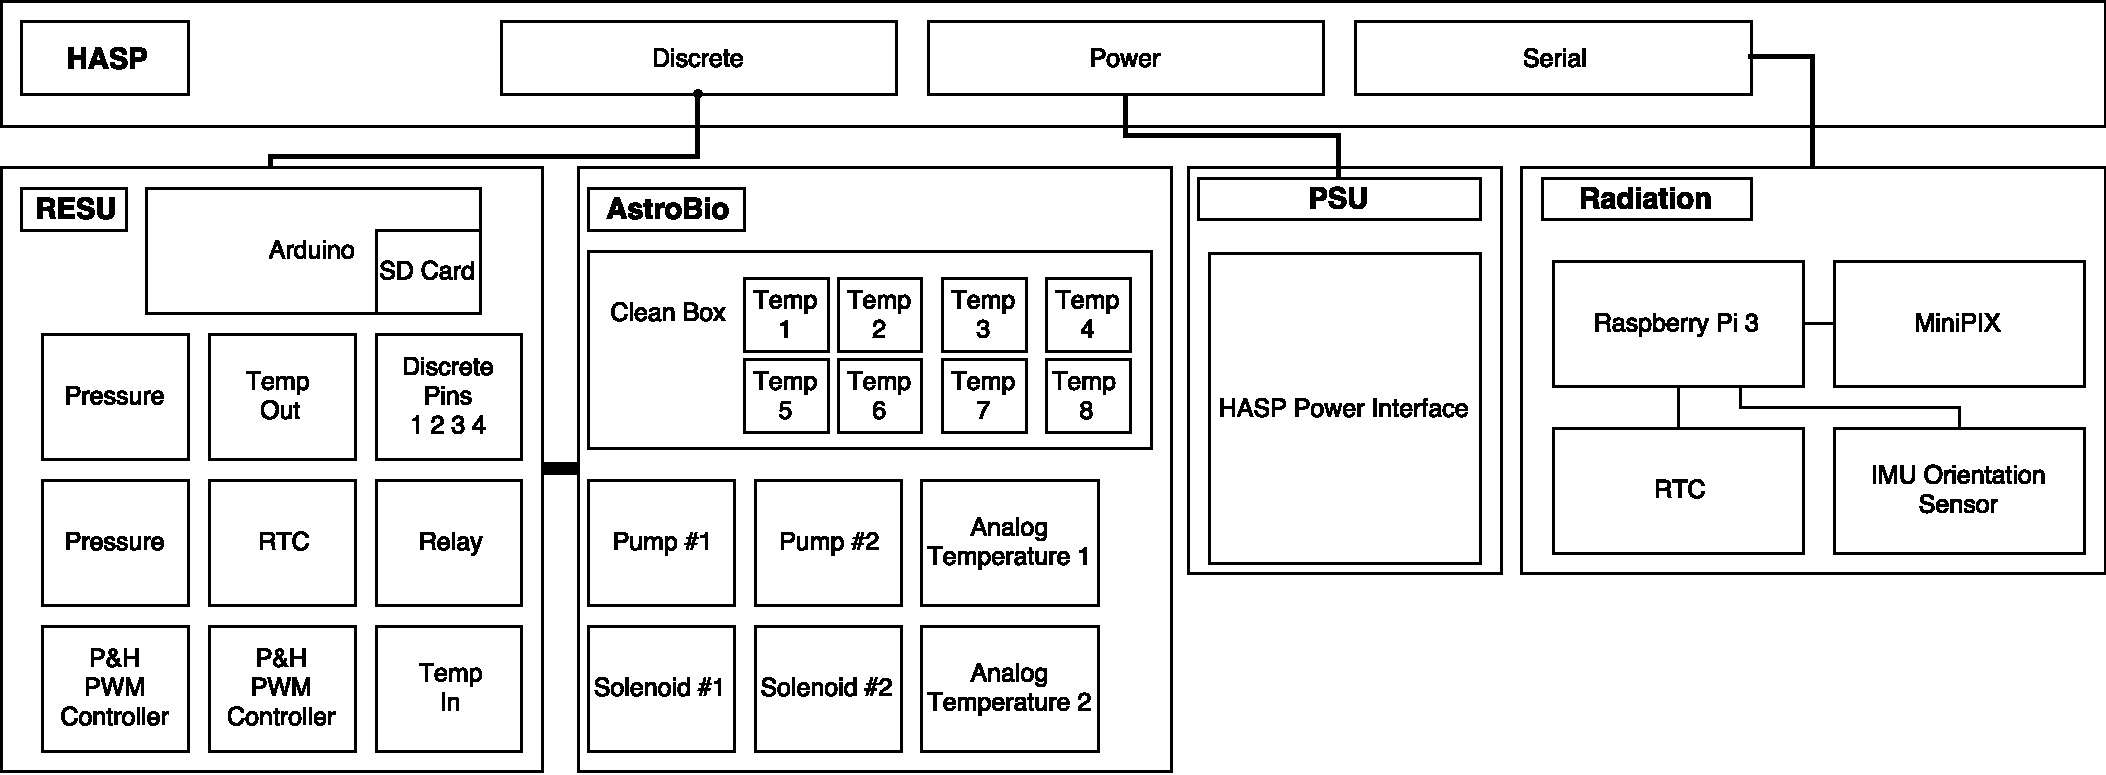
\includegraphics[width=\textwidth]{./Figures/RESU_2018.pdf}
\caption{Abstract subsystem design for SORA 2.0.}
\label{fig:payload} 
\end{center}
\end{figure}
